\section{Data Analysis}
\label{sec:4:data-analysis}
In this section, we present summary statistics and high-level illustrations of the transactions contained in the datasets of the three different blockchains.

\subsection{Transaction Overview}

% \point{Transaction volume}
% \autoref{fig:tx-usd-volume} shows the number of transactions and the transfer volume in USD that it represents. It is interesting to see that depending on the blockchain, the correlation between the number of transactions and the volume of money transferred varies vastly. Surprisingly, the correlation between these two metrics in XRP, which main's purpose is to transfer assets, is almost non-existent.

% \point{Transaction categories}
In~\autoref{fig:throughput-time}, we decompose the number of actions into different categories. XRPL and Tezos have well-defined action types, and we use the most commonly found ones to classify the throughput.
EOSIO does not have pre-defined action types: contract creators can decide on arbitrary action types.
To be able to classify the actions and understand where throughput on EOSIO is coming from, we manually label the top~\empirical{100} contracts, representing more than 99\% of the total throughput, by grouping them into different categories and assign one of the categories to each action.

\point{EOSIO}
Interestingly, there is a huge spike in the number of token actions from November 1, 2019, onward. 
We find that this is due to a new coin called \coin{EIDOS}~\cite{Enumivo2019} giving away tokens. 
We will describe this more extensively as a case study in Section~\ref{sec:eoscase}. 
Before this peak, the number of actions on EOSIO was vastly dominated by games, in particular betting games.

\point{Tezos}
Tezos has a high number of ``endorsements''---76\%, which are used as part of the consensus protocol, and only a small fraction of the throughput are actual actions.
It is worth noting that the number of ``endorsements'' should be mostly constant regardless of the number of transactions and that if the number of transactions were to increase enough, the trend would reverse.
We can also clearly see that Tezos has very regular spikes, with an interval of approximately two to three days each time.
These appear to be payments from bakers to stakers \cite{cryptium-labs-payout},\footnote{\url{https://twitter.com/CitezenB/status/1256147427905716224}} which can arguably be thought to be part of the consensus.
We use the TzKT API\footnote{\url{https://api.tzkt.io/}} to find account names and find that roughly \empirical{53\%} of these ``Transaction'' actions are sent by bakers and \empirical{6\%} of them are sent by the Tezos faucet~\cite{tezos-faucet}.
Endorsements and actions sent by either bakers or the faucet sum up about 87\% of the total number of actions.

\begin{figure}[tbp]
    \begin{subfigure}{\columnwidth}
        \centering
        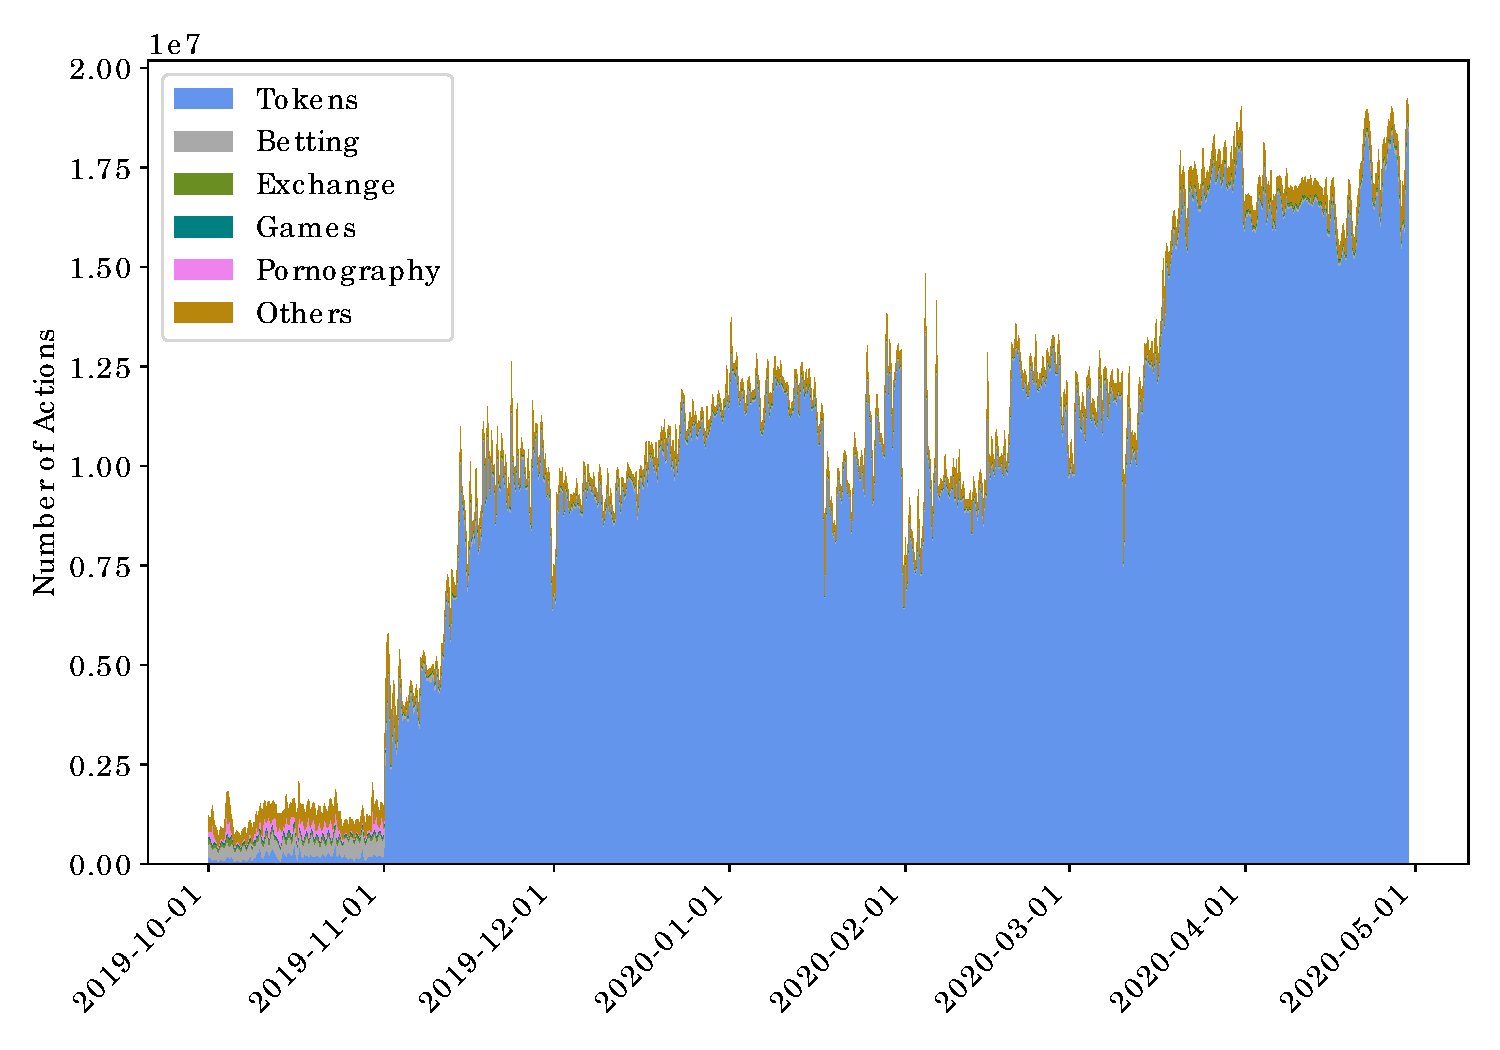
\includegraphics[height=.27\textheight]{./4-transactions-security/figures/eos-chart-area.pdf}
        \caption{EOSIO throughput over time}
        \label{fig:eos-throughput-time}
    \end{subfigure}
    \begin{subfigure}{\columnwidth}
        \centering
        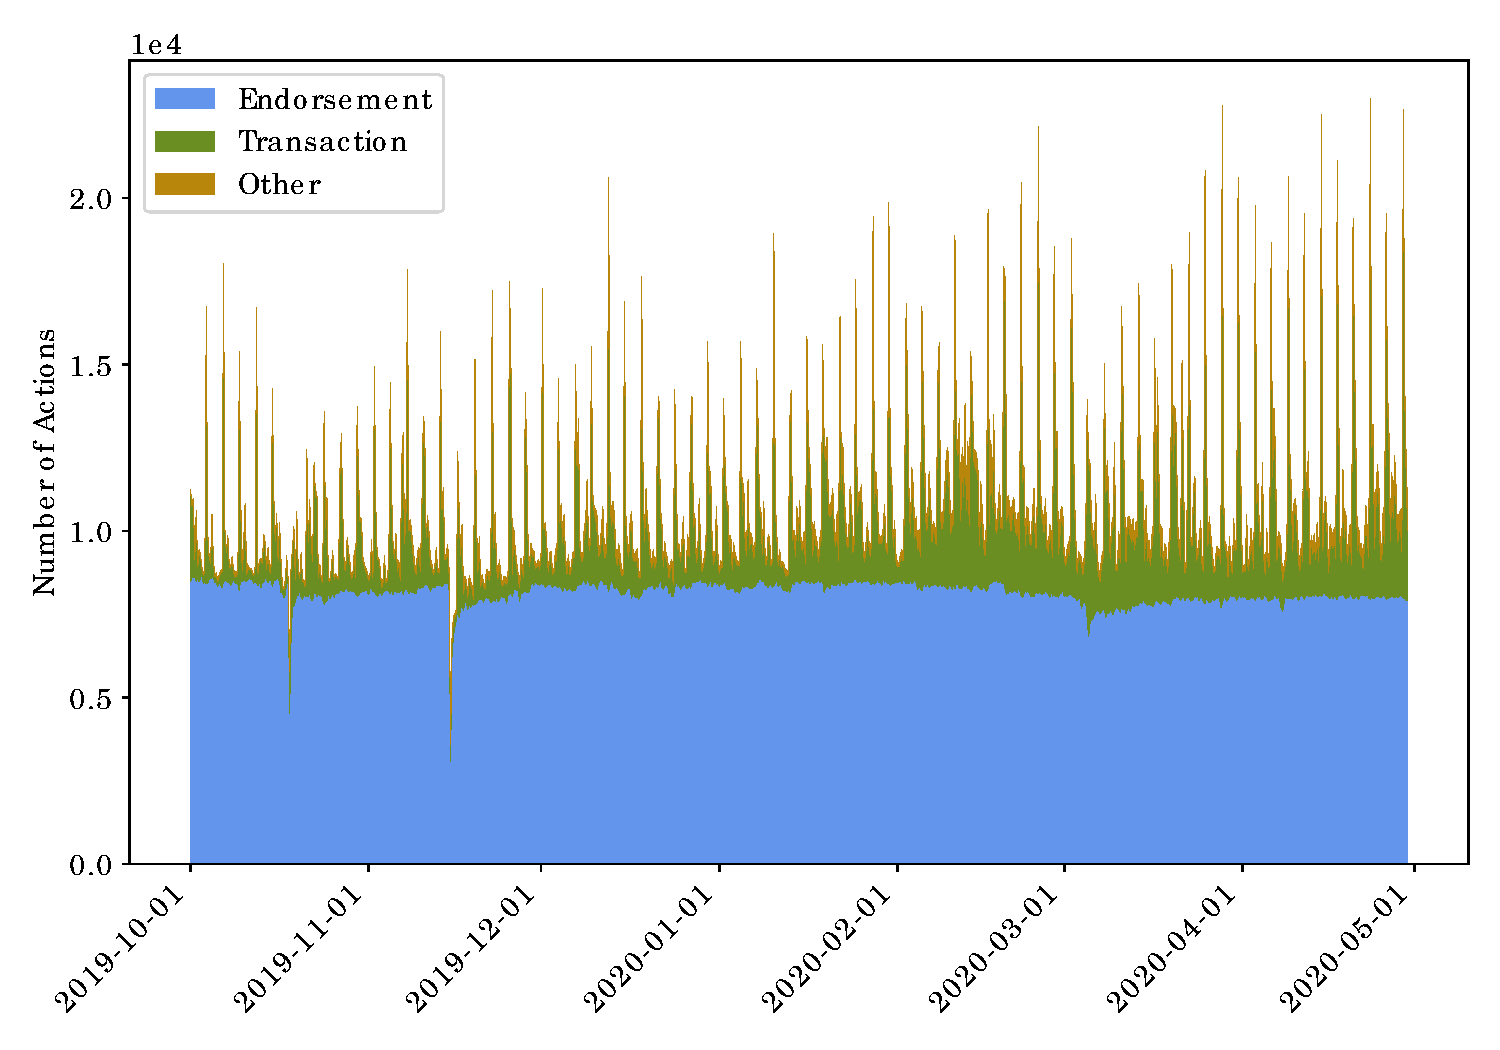
\includegraphics[height=.27\textheight]{./4-transactions-security/figures/tezos-chart-area.pdf}
        \caption{Tezos throughput over time}
        \label{fig:tezos-throughput-time}
    \end{subfigure}
    \begin{subfigure}{\columnwidth}
        \centering
        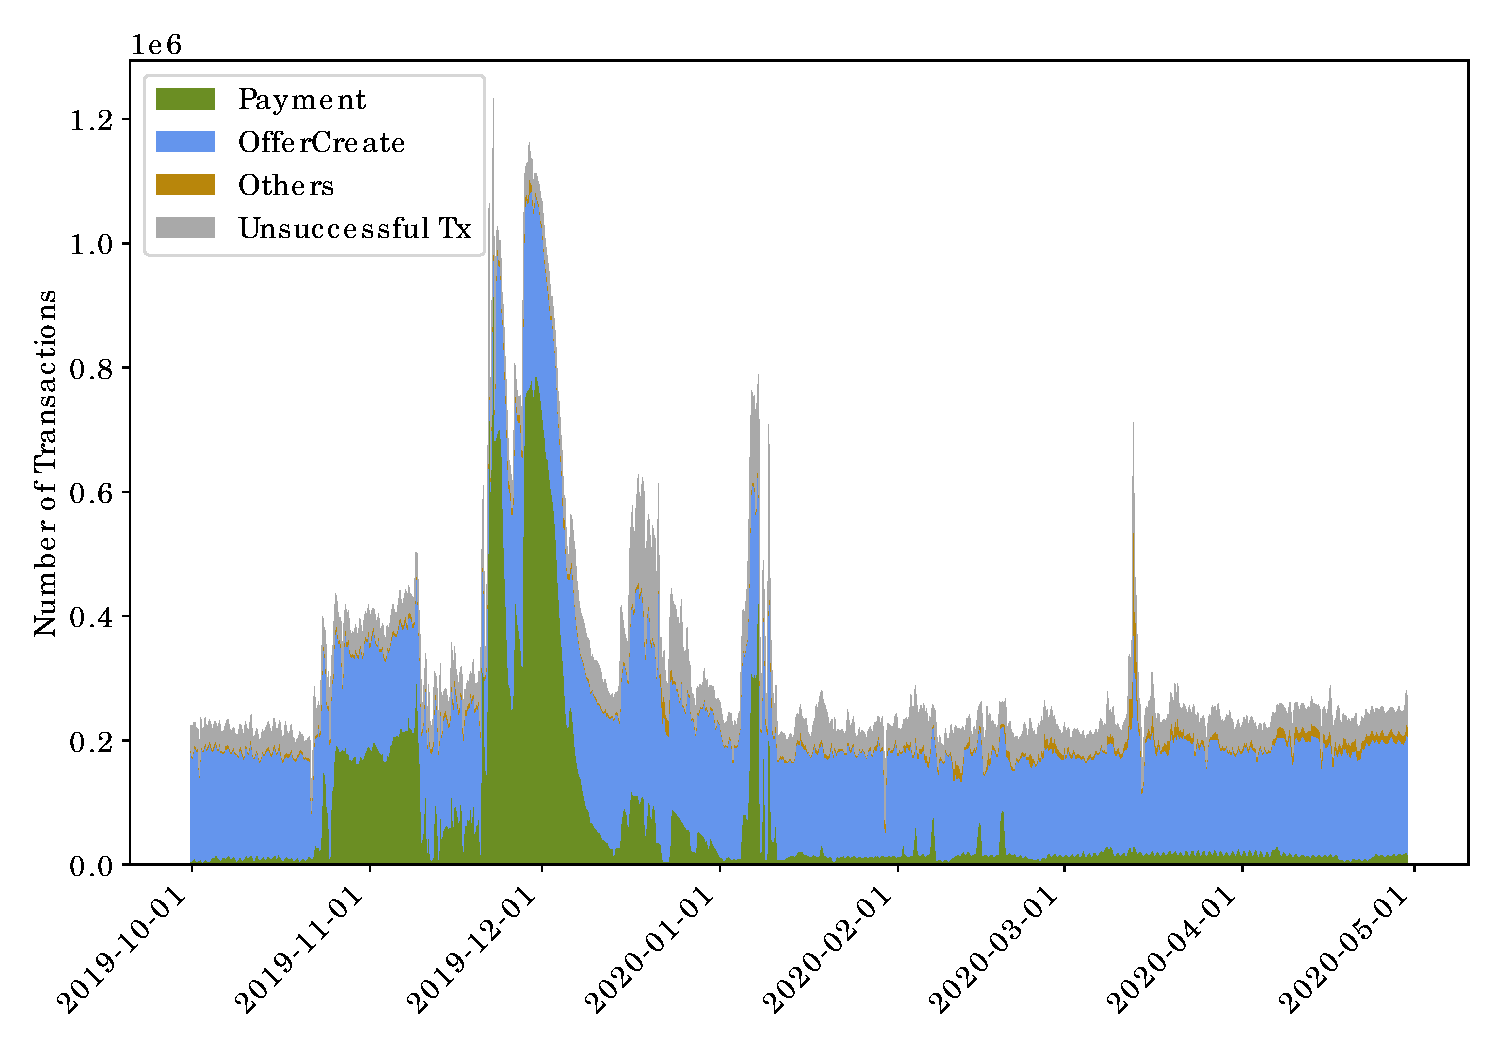
\includegraphics[height=.27\textheight]{./4-transactions-security/figures/xrp-chart-area.pdf}
        \caption{XRPL throughput over time}
        \label{fig:xrp-throughput-time}
    \end{subfigure}
    \caption[On-chain throughput over time]{On-chain throughput over time, the y-axis represents transaction count per 6 hours.}
    \label{fig:throughput-time}
\end{figure}

\begin{table}[tb]
    \centering
\caption[EOSIO top applications]{EOSIO top applications as measured using the number of received transactions.}
    \label{tab:eos-top-applications}
    \setlength{\tabcolsep}{2pt}
    \begin{tabular}{l l r l r}
    \toprule
    \textbf{Receiver} & \textbf{Description} & \textbf{Tx Count} & \multicolumn{2}{c}{\bf Actions}\\
         &         &    &  \bf Name   & \bf \% \\
    \midrule
      eosio.token & EOS token & 8,430,707,864 & transfer & 100.0\%\\
      \midrule
      \multirow{2}{*}{betdicetasks} & \multirow{2}{*}{Gambling game} & \multirow{2}{*}{32,804,674} & removetask & 66.65\%\\
                      & & & log & 15.71\%\\
      \midrule
      \multirow{3}{*}{whaleextrust} & \multirow{2}{*}{Decentralized} & \multirow{3}{*}{26,102,077} & verifytrade2 & 18.63\%\\
                      & & & verifytrade3 & 17.52\%\\
                      & exchange & & clearing & 16.77\%\\
      \midrule
      pptqipaelyog & Unknown & 24,109,437 & m & 93.00\%\\
      \midrule
      pornhashbaby & Pornography website & 23,677,938 & record & 99.86\%\\
    \bottomrule
    \end{tabular}
\end{table}


\point{XRPL}
On XRPL, both successful and unsuccessful transactions are recorded. A successfully executed transaction executes the command---such as \texttt{Payment}, \texttt{OfferCreate}, \texttt{OfferCancel}---specified by its initiator, while the only consequence of an unsuccessful transaction is the deduction of transaction fees from the transaction initiator.
Across the sample period, roughly~\empirical{one tenth} of transactions are unsuccessful (\autoref{fig:xrp-throughput-time}), with the most frequently registered errors being \texttt{PATH\_DRY} for \texttt{Payment} (insufficient liquidity, hence ``dry'', for specified payment path) and \texttt{tecUNFUNDED\_OFFER} for \texttt{OfferCreate} (no funds for the currency promised to offer by the offer creator). 

Successful transactions primarily consist of \texttt{Payment} (39.6\%) and \texttt{OfferCreate} (59.1\%) (\autoref{tab:transaction-types-distribution}). The number of \texttt{OfferCreate} is generally constant across time, but the number of \texttt{Payment} has a very high variance, with some periods containing virtually no payments and others having significant spikes. 
In Section \ref{sec:xrpcase}, we reveal why most transactions during these high-volume periods are economically meaningless. 

Except for the two spam periods, we observe that \texttt{OfferCreate} is the most common transaction type. 
Nonetheless, \texttt{OfferCreate} transactions contribute little to the total volume on XRPL.\footnote{
On May 10, 2020, for example, Ripple reported that the 24-hour XRP ledger trade volume---enabled via \texttt{OfferCreate} transactions---only accounts for \empirical{1\%} of the total ledger volume, while the payment volume---enabled via \texttt{Payment} transactions---accounts for \empirical{99\%}.
} This is because an offer expires if not fulfilled (fully or partially) before the expiry time defined by the offer creator; it can also be cancelled by its creator or superseded by a new offer. In fact, \empirical{0.2\%} of \texttt{OfferCreate} transactions resulted in an actual token exchange deal during our observation period. 


% With exchanges in the conventional financial market, transaction fees are only levied for matched offers; with decentralized
% exchanges (DEX) on XRPL, in contrast, every offer placed through \texttt{OfferCreate}, whether or not fulfilled, is broadcasted on the network, recorded on the ledger as a transaction and counts towards the overall throughput, and hence incurs a transaction fee.

% While the official XRP Charts may exclude transactions that Ripple believes not to be ``bona fide'', Ripple does not seem to have exerted censorship. To a very large extent, the results from independent exploration of XRPL data align well with Ripple's charts \cite{Ripple2020}. 



% As a result, balances of accounts involved are recalculated, and, when applicable, states of decentralized exchanges are updated accordingly. Conversely, the sole consequence of an unsuccessful transaction is the deduction of transaction fees from the transaction initiator.
 
% To calculate transaction volume is non-trivial on the XRP ledger. Value exchange does not only triggered by transaction type \texttt{Payment}, but also by \texttt{OfferCreate}. A created offer can be non-fulfilled, partially fulfilled or fully fulfilled.

% To measure the value exchange triggered by \texttt{OfferCreate}, we extract the information on how an \texttt{AccountRoot} is modified and calculated the difference in balance between before and after the transaction. 


\subsection{Transaction Patterns}
To understand better what the major sources of traffic constitute, we analyze the top accounts on EOSIO, Tezos, and XRPL, and find various transaction patterns.

\point{EOSIO}
In \autoref{tab:eos-top-applications}, we show EOSIO accounts with the highest number of received actions.
We can see that the \texttt{eosio.token} account, which is the account used to handle \coin{EOS} token transfers, is by far the most used, and almost all calls to this account use the \texttt{transfer} action.
Although \coin{EOS} transfers are indeed a central part of the EOSIO ecosystem, more than~\empirical{99.9}\% of the transfers shown are exclusively to and from this EIDOS account.
The second account is a betting website where all the bets are performed transparently using EOSIO.
However, around~\empirical{80\%} of the actions---\texttt{removetask} and \texttt{log}---are bookkeeping, and the actual betting-related actions such as \texttt{betrecord} represent a very low percentage of the total number of actions.
The third account is a decentralized exchange and is used to exchange different assets available on EOSIO. This exchange will be discussed in Section~\ref{sec:case-studies}.
We could not find information about the fourth account, but it is very actively sending \coin{EOS} tokens to the EIDOS account.
Finally, the last account was a pornography website which used EOSIO as a payment system. This account is still the fifth account with the highest number of received actions although the service was discontinued in November 2019 for financial reasons~\cite{hashbaby-closing}.

\begin{table}
    \caption{Tezos accounts with the highest number of sent transactions.}
    \label{tab:tezos-account-edges}
    \centering
    \setlength{\tabcolsep}{1.4pt}
    \begin{tabular}{@{}l r r r@{}}
    \toprule
               &            &           & \bf Avg. \# of\\
               & \bf Sent         & \bf Unique    & \bf transactions\\
    \bf Sender & \bf count & \bf receivers & \bf per receiver\\
    \midrule
    \tezaddr{tz1VwmmesDxud2BJEyDKUTV5T5VEP8tGBKGD} & 106,477 & 23,649 & 4.50\\
    \tezaddr{tz1cNARmnRRrvZgspPr2rSTUWq5xtGTuKuHY} & 105,202 & 2,096 & 50.19\\
    \tezaddr{tz1Mzpyj3Ebut8oJ38uvzm9eaZQtSTryC3Kx} & 93,448 & 93,444 & 1.00\\
    \tezaddr{tz1SiPXX4MYGNJNDsRc7n8hkvUqFzg8xqF9m} & 57,841 & 19,382 & 2.98\\
    \tezaddr{tz1acsihTQWHEnxxNz7EEsBDLMTztoZQE9SW} & 42,683 & 1,436 & 29.72\\
    \bottomrule
    \end{tabular}
\end{table}


\point{Tezos}
As Tezos neither has account names nor actions in the transaction metadata, analysing the top receivers' accounts is less interesting, as it is very difficult to perform any type of attribution. However, we find interesting patterns from observing the top sending accounts.
Most of the top senders in Tezos seem to follow a similar pattern: Sending a small number of transactions (between~\empirical{5} and~\empirical{50}) to many different accounts. 
Another important thing to note is that all of these accounts are not contracts but regular accounts, which means that the transactions are automated by an off-chain program.
After further investigation, we find that the top address is the Tezos Faucet~\cite{tezos-faucet}. The other addresses appear to be bakers' payout addresses and the transactions are payouts to stakers~\cite{backerei}, corresponding to the peaks seen in~\autoref{fig:tezos-throughput-time}. For completeness, we include the top senders and some statistics about them in \autoref{tab:tezos-account-edges}.

\point{XRPL}
% top_acct.pkl
From \startdate to \finishdate, a total of~\empirical{195 thousand} accounts collectively conducted~\numprint{\fpeval{\XRPcount/1000000}} million transactions, i.e. an average of~\empirical{1.4 thousand} transactions per account during the seven-month observation period.

The distribution of the number of transactions per account is highly skewed. 
\empirical{Over one third~(71 thousand)} of the accounts have transacted only once during the entire observation period, whereas the~\empirical{35} most active accounts are responsible for half of the total traffic. 
\autoref{tab:xrpspammers} lists of the top~10 accounts by the number of conducted transactions. 
With the exception of \xrpaddr{rKLpjpCoXgLQQYQyj13zgay73rsgmzNH13} and \xrpaddr{r96HghtYDxvpHNaru1xbCQPcsHZwqiaENE}, all these accounts share suspiciously similar patterns:
\begin{enumerate}
    \item more than~98\% of their transactions are \texttt{OfferCreate};
    \item they are either descendants of an account from \href{https://www.huobi.com/}{Huobi}, a crypto exchange founded in China, or frequently transact with descendants from Huobi;
    \item they have all transacted using \coin{CNY};
    \item their payment transactions conspicuously use the same destination tag \texttt{104398}, a field that---similar to a bank reference number---exchanges and gateways use to specify which client is the beneficiary of the payment~\cite{XRPLedger2020b}.
\end{enumerate}
%
The aforementioned similarities, in particular the last one, signal that those accounts are controlled by the same entity, presumably with a strong connection to Huobi. 
The frequent placement of offers might come from the massive client base of the entity.

Notably, the sixth most active account, \xrpaddr{r96HghtYDxvpHNaru1xbCQPcsHZwqiaENE}, registered under the username \texttt{chineseyuan} only carried out \textit{one} successful \texttt{Payment} transaction during the observation period, while the rest of the over four million transactions failed with a \texttt{PATH\_DRY} error. Recall that failed transactions still occupy on-chain throughput. Therefore, it is evident that \texttt{chineseyuan} spammed the network.

\begin{table}[ht]
	\centering
	\caption{XRPL accounts with the highest number of transactions.}
	\label{tab:xrpspammers}%
	\footnotesize
	\renewcommand{\arraystretch}{0.6}
	\setlength{\tabcolsep}{3pt}
	\begin{tabular}{llrrrr}
		\toprule
		\textbf{Account}                                                 & \textbf{Type} & \textbf{ Count } &  & \textbf{ TotalCount }                                     & \textbf{\% of throughput}  \\
		\midrule
		\multirow{3}[0]{*}{\xrpaddr{r4AZpDKVoBxVcYUJCWMcqZzyWsHTteC4ZE}} & OfferCreate   & 21,790,612       &  & \multicolumn{1}{r}{\multirow{3}[0]{*}{      22,082,431}}  & \multirow{3}[0]{*}{8.13\%} \\
		                                                                 & Others        & 291,687          &  &                                                           &                            \\
		                                                                 & Payment       & 132              &  &                                                           &                            \\
		\midrule
		\multirow{3}[0]{*}{\xrpaddr{rQ3fNyLjbvcDaPNS4EAJY8aT9zR3uGk17c}} & OfferCreate   & 21,716,850       &  & \multicolumn{1}{r}{\multirow{3}[0]{*}{      21,856,984}}  & \multirow{3}[0]{*}{8.05\%} \\
		                                                                 & Others        & 140,088          &  &                                                           &                            \\
		                                                                 & Payment       & 46               &  &                                                           &                            \\
		\midrule
		\multirow{3}[0]{*}{\xrpaddr{rh3VLyj1GbQjX7eA15BwUagEhSrPHmLkSR}} & OfferCreate   & 21,510,597       &  & \multicolumn{1}{r}{\multirow{3}[0]{*}{      21,541,929}}  & \multirow{3}[0]{*}{7.93\%} \\
		                                                                 & Others        & 31,295           &  &                                                           &                            \\
		                                                                 & Payment       & 37               &  &                                                           &                            \\
		\midrule
		\multirow{3}[0]{*}{\xrpaddr{r4dgY6Mzob3NVq8CFYdEiPnXKboRScsXRu}} & OfferCreate   & 21,474,131       &  & \multicolumn{1}{r}{\multirow{3}[0]{*}{      21,504,135}}  & \multirow{3}[0]{*}{7.92\%} \\
		                                                                 & Others        & 29,841           &  &                                                           &                            \\
		                                                                 & Payment       & 163              &  &                                                           &                            \\
		\midrule
		\xrpaddr{rKLpjpCoXgLQQYQyj13zgay73rsgmzNH13}                     & Payment       & 4,493,754        &  & \multicolumn{1}{r}{        4,493,754 }                    & 1.65\%                     \\
		\midrule
		\xrpaddr{r96HghtYDxvpHNaru1xbCQPcsHZwqiaENE}                     & Payment       & 4,488,127        &  & \multicolumn{1}{r}{        4,488,127 }                    & 1.65\%                     \\
		\midrule
		\multirow{2}[0]{*}{\xrpaddr{rBW8YPFaQ8WhHUy3WyKJG3mfnTGUkuw86q}} & OfferCreate   & 4,474,481        &  & \multicolumn{1}{r}{\multirow{2}[0]{*}{        4,475,448}} & \multirow{2}[0]{*}{1.65\%} \\
		                                                                 & Others        & 967              &  &                                                           &                            \\
		\midrule
		\multirow{2}[0]{*}{\xrpaddr{rDzTZxa7NwD9vmNf5dvTbW4FQDNSRsfPv6}} & OfferCreate   & 4,472,749        &  & \multicolumn{1}{r}{\multirow{2}[0]{*}{        4,473,792}} & \multirow{2}[0]{*}{1.65\%} \\
		                                                                 & Others        & 1,043            &  &                                                           &                            \\
		\midrule
		\multirow{3}[0]{*}{\xrpaddr{rV2XRbZtsGwvpRptf3WaNyfgnuBpt64ca}}  & OfferCreate   & 4,470,525        &  & \multirow{3}[0]{*}{        4,471,578}                     & \multirow{3}[0]{*}{1.65\%} \\
		                                                                 & Others        & 977              &  &                                                           &                            \\
		                                                                 & Payment       & 76               &  &                                                           &                            \\
		\midrule
		\multirow{3}[0]{*}{\xrpaddr{rwchA2b36zu2r6CJfEMzPLQ1cmciKFcw9t}} & OfferCreate   & 4,470,528        &  & \multirow{3}[0]{*}{        4,471,551}                     & \multirow{3}[0]{*}{1.65\%} \\
		                                                                 & Others        & 1,008            &  &                                                           &                            \\
		                                                                 & Payment       & 15               &  &                                                           &                            \\
		\bottomrule
	\end{tabular}%
\end{table}


\subsection{Analysis Summary}
Here, we highlight some of the observations about the data described above. 
\begin{itemize}\itemsep=0pt
    \item Transactions on EOSIO can be roughly divided by the category of contracts they belong to. 
    Before the arrival of the \coin{EIDOS} token, approximately~\empirical{50\%} of these are transactions to betting games. The rest was split between token transfers and various forms of entertainment, such as games not involving betting as well as payments to pornography websites. The launch of \coin{EIDOS} increased the total number of transactions more than tenfold, resulting in~\empirical{96\%} of the transactions being used for token transfers.
    
    \item The vast majority~(\empirical{76}\%) of transactions on Tezos are used by the \texttt{endorsement} operation to maintain consensus. This is because blocks typically contain 32 endorsements~\cite{Tezos2018} and the number of transactions on the network is still low. The rest of the throughput is mainly used by transactions to transfer assets between accounts.
    
    \item \texttt{OfferCreate} and \texttt{Payment} are the two most popular transaction types on XRPL, accounting for \empirical{59.1\%} and~\empirical{36.9\%} of the total throughput, respectively. Between \startdate and October 8, 2019, before the systematic spamming periods, the fractions of \texttt{OfferCreate} and \texttt{Payment} are \empirical{79\%} and \empirical{18\%}, respectively. Overall, \empirical{one-tenth} of the transactions fail.
\end{itemize}
